\documentclass[TFG.tex]{subfiles}

\begin{document}


%\hyphenation{equi-va-len-cia}\hyphenation{pro-pie-dad}\hyphenation{res-pec-ti-va-men-te}\hyphenation{sub-es-pa-cio}
\chapter{Automorfismos del grupo libre}

Vamos a empezar este capítulo dando otra interpretación de los grupos de trenzas. Aunque originalmente Artin visualizó las trenzas como una colección de cuerdas, existe una representación natural como automorfismos del grupo libre $F_n$ de rango $n$. Definiremos esta representación por medio de \emph{mapping classes}.

\section{Representación del grupo de trenzas como automorfismos del grupo libre}

\begin{figure}[h!]
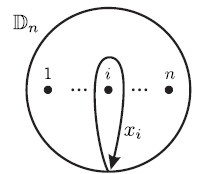
\includegraphics[scale=0.7]{Imagenes/Disco.png}
\caption{Los lazos $x_1,\dots,x_n$ son generadores de $\pi_1(\D_n)$.}\label{disco}
\end{figure}

Observamos que el grupo fundamental del disco agujereado $n$ veces, $\D_n$, es precisamente el grupo libre de rango $n$, es decir, $\pi_1(\D_n)=F_n$. Si fijamos un punto base, digamos, en el borde del disco, podemos tomar como generadores los lazos $x_1,\dots, x_n$ descritos en la Figura \ref{disco}. Ahora, una trenza $\beta\in B_n$ puede ser vista como un automorfismo de $\D_n$ que es la identidad en el borde $\partial(\D_n)$ salvo isotopía (que también fija los puntos de $\partial(\D_n)$), así que $\beta$ induce una acción bien definida sobre $\pi_1(\D_n)=F_n$, donde un lazo $\gamma\in\pi_1(\D_n)$ es enviado a $\beta(\gamma)$. Esta acción es claramente un homomorfismo de grupos (respeta la concatenación), %igual esto debería intentar comprobarlo cuando entienda lo de los mapping class mejor 
el cual es biyectivo pues $\beta^{-1}$ da lugar a la acción inversa. Entonces, $\beta$ induce un automorfismo de $F_n$, y esto nos da la representación
%\[
%\begin{tikzcd}
%\rho: B_n\ \arrow[r] & Aut(F_n)\\
%       \beta\arrow[r,mapsto,shorten >= 1em, shorten <= 1em] & \rho_\beta.
%\end{tikzcd}
%\]
\begin{align*}
\rho: & B_n \to Aut(F_n)\\
      & \beta\ \ \mapsto\ \ \rho_\beta.
\end{align*}
El automorfismo $\rho_\beta$ puede ser descrito fácilmente cuando $\beta=\sigma_i$, dando la imagen de los generadores $x_1,\dots, x_n$ de $F_n$ (ver Figura \ref{auto}), esto es:
$$\rho_{\sigma_i}(x_i)=x_{i+1},\quad \rho_{\sigma_i}(x_{i+1})=x_{i+1}^{-1}x_ix_{i+1},\quad \rho_{\sigma_i}(x_j)=x_j\ (j\neq i,i+1).$$
El automorfismo $\rho_{\sigma_i^{-1}}=\rho^{-1}_{\sigma_i}$ puede ser deducido fácilmente a partir de $\rho_{\sigma_i}$, lo que nos da
$$\rho^{-1}_{\sigma_i}(x_i)=x_ix_{i+1}x_i^{-1},\quad \rho^{-1}_{\sigma_i}(x_{i+1})=x_i,\quad \rho^{-1}_{\sigma_i}(x_j)=x_j\ (j\neq i,i+1).$$
Para una trenza general $\beta$, escrita como producto de $\sigma_1,\dots,\sigma_{n-1}$ y sus inversas, el automorfismo $\rho_\beta$ es simplemente la composición de los correspondientes automorfismos inducidos por cada letra.

\begin{figure}[h!]
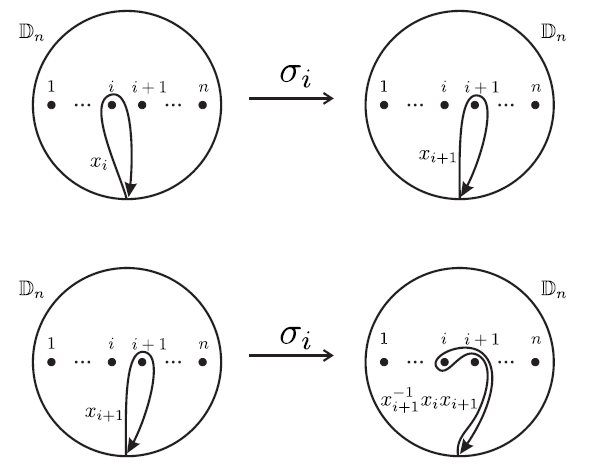
\includegraphics[scale=0.7]{Imagenes/auto.png}
\caption{Acción de $\sigma_i$ sobre los generadores $x_i$ y $x_{i+1}$.}\label{auto}
\end{figure}

Es fácil ver que $\rho$ está bien definido algebraicamente, ya que $\rho_{\sigma_i\sigma_j}=\rho_{\sigma_j\sigma_i}$ si $|i-j|>1$, y $\rho_{\sigma_i\sigma_j\sigma_i}=\rho_{\sigma_j\sigma_i\sigma_j}$ si $|i-j|=1$. 




\begin{teorema}
La representación anterior es fiel, es decir, dos trenzas están representadas por el mismo automorfismo si y solo si son la misma.
\end{teorema}

La prueba de este resultado se puede encontrar en \cite{Birman}. Lo significativo ahora es que esta representación nos permite resolver el problema de la palabra como explicaremos a continuación.

\newpage

\section{Solución al problema de la palabra}
El hecho de que las trenzas puedan ser vistas fielmente como automorfismos del grupo libre $F_n$ da lugar inmediatamente a una solución al problema de la palabra en $B_n$. Dadas dos trenzas $\beta_1$ y $\beta_2$, expresadas como palabras en $\sigma_1,\dots,\sigma_{n-1}$ y sus inversas, se pueden calcular sus correspondientes automorfismos $\rho_{\beta_1}$ y $\rho_{\beta_2}$. Entonces $\beta_1=\beta_2$ si y solo si $\rho_{\beta_1}\equiv \rho_{\beta_2}$, lo cual ocurre si y solo si $\rho_{\beta_1}(x_i)= \rho_{\beta_2}(x_i)\in F_n$ para $i=1,\dots, n$. Como el problema de la palabra en $F_n$ tiene solución conocida (basta calcular las palabras reducidas asociadas a $\rho_{\beta_1}(x_i)$ y $\rho_{\beta_2}(x_i)$), esto resuelve el problema de la palabra en $B_n$. 

Merece la pena remarcar que este algoritmo no es en absoluto eficiente (de hecho tiene complejidad exponencial) y existen otros que lo son mucho más, pero esta es históricamente la primera solución conocida para el problema de la palabra en $B_n$, descubierta por Artin y publicada en \cite{ArtinA}.

Veamos un ejemplo de cómo se aplica este método.
\begin{ej}
Dado $n\geq 3$, sean $\beta_1=\sigma_i\sigma_{i+1}^{-1}\sigma_i$ y $\beta_2=\sigma_{i+1}\sigma_i^{-1}\sigma_{i+1}$ para algún $1\leq i\leq n-2$. Nos preguntamos si estas palabras representan la misma trenza. Serán la misma si y solo si $\rho_{\beta_1}(x_j)=\rho_{\beta_2}(x_j)$ para todo $1\leq j\leq n-1$, por lo que para probar que son distintas basta encontrar un generador del grupo libre para el que sus imágenes no coincidan. Sea pues $x_i$. Tenemos por un lado
$$\rho_{\beta_1}(x_i)=\rho_{\sigma_i}(x_i)\rho^{-1}_{\sigma_{i+1}}(x_i)\rho_{\sigma_i}(x_i)=
x_{i+1}x_ix_{i+1}$$
y por otro
$$\rho_{\beta_2}(x_i)=\rho_{\sigma_{i+1}}(x_i)\rho_{\sigma_i}^{-1}(x_i)\rho_{\sigma_{i+1}}(x_i)=
x_i (x_i x_{i+1} x_i^{-1})x_i=x_i^2x_{i+1}.$$
Claramente $x_{i+1}x_ix_{i+1}\neq x_i^2x_{i+1}$ en $F_n$, por lo que $\beta_1\neq\beta_2$.
\end{ej}

\end{document}